\section{Retrieval model}
\label{sec:retrieval_model}
\subsection{Overview}
\begin{figure}[!htb]
    \centering
    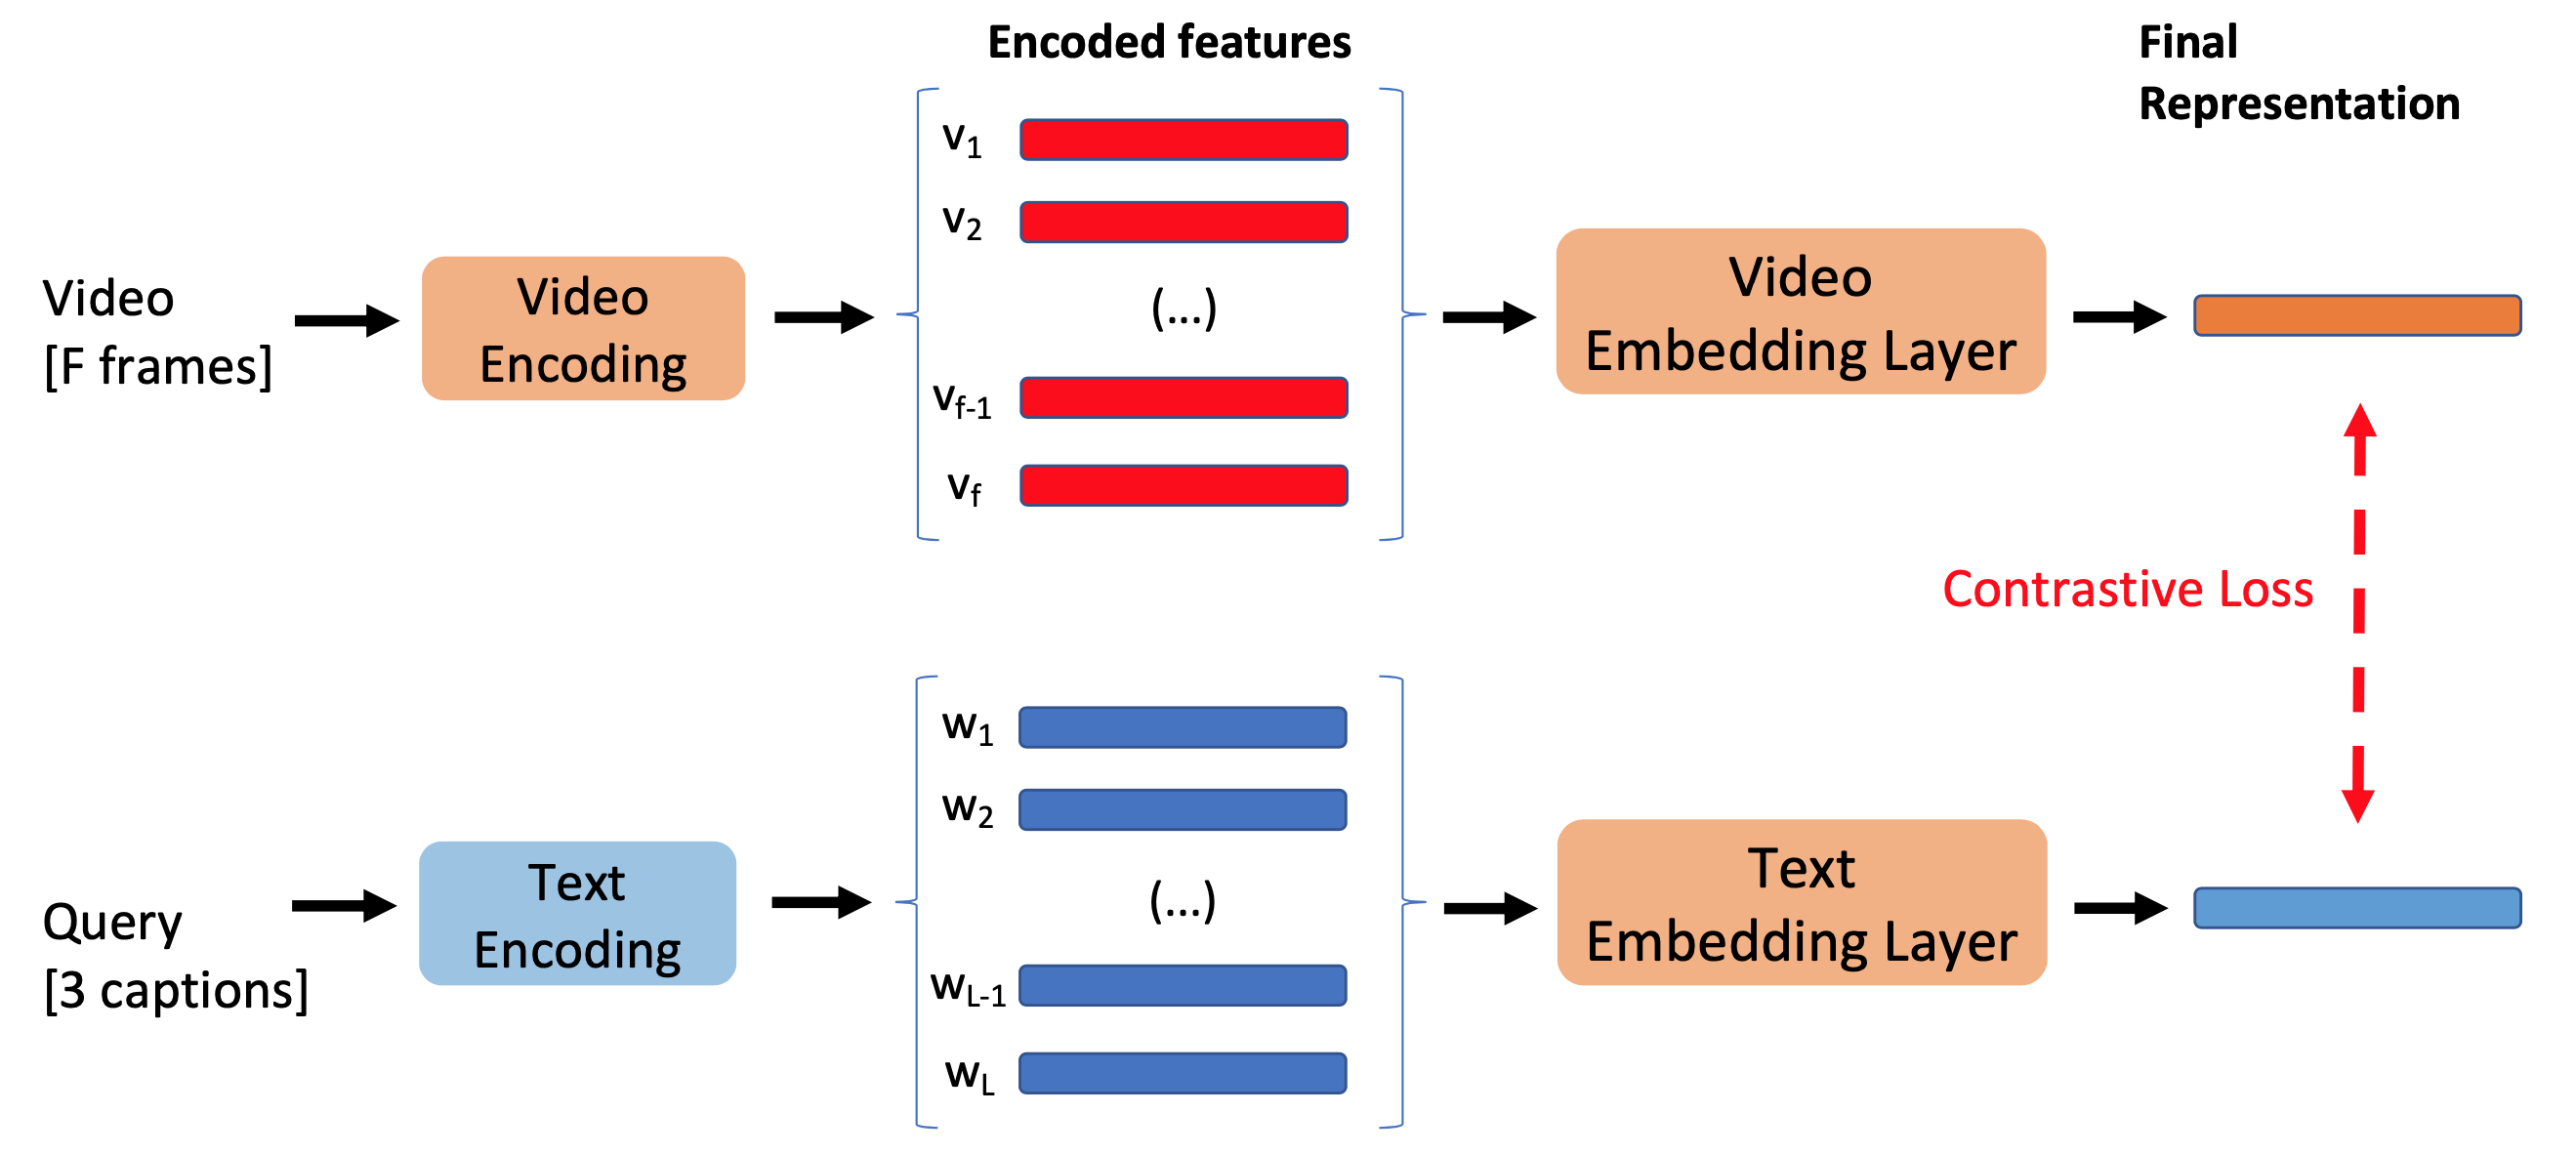
\includegraphics[width=\linewidth]{resources/images/methods/retrieval_model.png}
    \caption{Retrieval model architecture.}
    \label{fig:ret_overview}
\end{figure}
Representation learning-based (RL-based) retrieval methods have shown potential results in various modalities. 
Especially for sequential data such as video and text, the attention mechanism provides a powerful technique for rich feature extraction, which leads to many success in cross-modalities learning tasks (as discussed in section \ref{sec:video-text_ret}). 
To efficiently apply this method to the vehicle-based retrieval problem, we employ a transformer-based architecture to learn the representation for video and text input, in which, the video encoded input is constructed from the target's essential appearance features. 
We inherit the embedding backbone of the COOT framework \cite{ging2020coot}, with some modification for better fit with our scenario.
Figure \ref{fig:ret_overview} summarizes our proposed approach.

\subsection{Representation learning}
\subsubsection{Query encoding [TODO: attribute-aware]}
In text branch, we can naively model the paragraph input in many different ways by choosing one from the combinations of three different sentences for each query.
However, we observe that the three descriptions can contain mutual meaning. For instance, the later caption may have reference to the former one.
\begin{itemize}
    \item \textit{\underline{Yellow car} keeps straight.}
    \item \textit{\underline{A yellow coupe} keeps straight before a diverging road.}
    \item \textit{There was a black pickup behind \underline{the vehicle}.}
\end{itemize}
Thus, in the encoding step, we aim to concatenate those descriptions as a whole paragraph, which provides the complete information for a specific target track.
For a query $q_i = [s_{i=1:3}]$, the preparing process is setup as follow:
\begin{enumerate}
    \item Splitting each sentence $s_i$ into a list of tokens.
    \item Encoding each token to a $d_{word}$-dimension vector. Consequently, the sentence vector is therefore a list of word vectors.
    \item Concatenating the three-sentence vectors as a final representation $\mathbf{v_{query}}$ for the query.
\end{enumerate}

\subsubsection{Video encoding}
In video branch, the video track also contains the local information of the target vehicle, which is usually the main subject and provides potential visual attributes described in the given query. For that reason, different from the original COOT method, we also include the target's attribute features in the video encoding vector. \\
In the COOT framework, given a video $V$ with $F$ frames, the video encoding is constructed by concatenating all $F$ frame-level feature $d_F$-dimension vectors, which are extracted by pretrained backbones.
For each frame, the feature vectors, enriched by deep neural networks pretrained on large benchmark datasets, contain helpful global information but lack local ones, which could be the target vehicles we need to focus on in the CityFlow-NL setup. 
From this point of view, we modify the frame-level encoded vectors with the following strategy.
Let $\mathbf{v_{frame}}$ denotes the feature vector for each frames in a video track, $\mathbf{v_{frame}} \in \mathbb{R}^{d_f}$. We define this feature as a combination of three sources:
\begin{enumerate}
    \item \textbf{Global context information ($\mathbf{v_{global}}$)}. The element aim to provide general information of each video frame.
    \item \textbf{Attributes representation ($\mathbf{v_{veh}}$)}. The compact feature produced by the attribute classifiers (section \ref{sec:vehcol_extraction}) provides the important details of the target vehicle that the model needs to focus on during the retrieval process.
    \item \textbf{Target vehicle location ($\mathbf{v_{loc}}$)}. The relative location and size of target vehicle at each time step, provide the main subject's movement trajectory information.
\end{enumerate}
For the $\mathbf{v_{global}}$, we apply the same approach as the COOT framework, which is the global feature extracted by the ResNet-152 \cite{he2016deep} pretrained on ImageNet \cite{russakovsky2015imagenet}. 
The $\mathbf{v_{veh}}$ is constructed as a concatenation of color and vehicle-type encoded vectors ($\mathbf{v_{veh-col}}$, $\mathbf{v_{veh-type}}$) provided by the corresponding encoders $E_{col}$ and $E_{veh}$, details in \ref{sec:vehcol_extraction}.
\[ 
\mathbf{v_{veh}} = concat(\mathbf{v_{veh-col}}, \mathbf{v_{veh-type}})
\]
And the vehicle location component is constructed from the bounding box coordinates at a given frame.
\[
\mathbf{v_{loc}} = [x/W, y/H, w/W, h/H]
\]
where $(x, y, w, h)$ denotes the box top-left coordinate, width, height. $(W, H)$ are respectively the width, height of the video frame. 
\begin{figure}[!h]
    \centering
    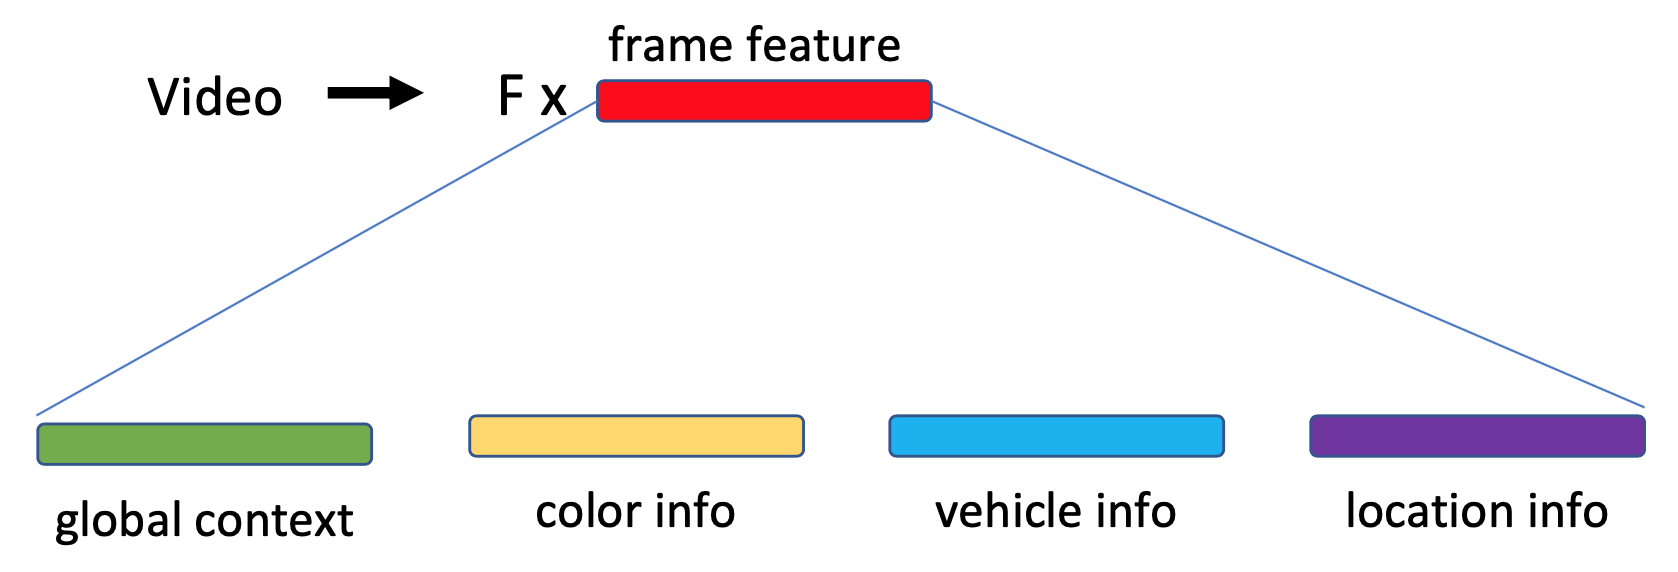
\includegraphics[width=\linewidth]{resources/images/methods/video_encoding.png}
    \caption{Video encoding procedure.}
    \label{fig:video_encoding}
\end{figure}

In total, the frame encoded feature is modelled as:
\[
\mathbf{v_{frame}} = concat(\mathbf{v_{global}}, \mathbf{v_{veh}}, \mathbf{v_{loc}})
\]
which contains both global context and target's descriptive informations. And the final encoding for each F-length video track $\mathbf{v_{track}}$ is the combination of F frame-level features, resulting in $F \times d_f$-dimension vector (illustrated in Figure \ref{fig:video_encoding}).
The track/query representation feature ($\mathbf{v_{track}}$, $\mathbf{v_{query}}$) is then fed forward through the corresponding encoding blocks to obtain the final embedding vectors.

\subsection{Loss function}
To efficiently train the retrieval model, we inherent the alignment loss of Zhang et al. \cite{zhang2018cross}, which leverage the contrastive loss to enforce the positive samples to stay closer and the negative ones far apart. 
Given a positive sample $P = (q_i, v_i)$, set of two negative pairs $N = \{({q_i}', v_i), (q_i, {v_i}')\}$ and a margin $\alpha$, they define the following loss:
\begin{equation}
\begin{split}
    L(P, N, \alpha) = & \mathrm{max}(0, \alpha + D(q_i, v_i) - D({q_i}', v_i)) + \\ 
    & \mathrm{max}(0, \alpha + D(q_i, v_i) - D(q_i, {v_i}'))
\end{split}
\end{equation}
% \begin{align}
%     L(P, N, \alpha) = & \mathrm{max}(0, \alpha + D(q_i, v_i) - D({q_i}', v_i)) + \\ 
%     & \mathrm{max}(0, \alpha + D(q_i, v_i) - D(q_i, {v_i}'))
% \end{align}
Where $D(x, y) = 1 - \frac{x^{\top}y}{\left \| x \right \|\left \| y \right \|}$ denotes the cosine distance between two representation vectors, $q_i$ and $v_i$ indicate the embedding vectors of query and video respectively. \\
The alignment loss is defined as follow.
\begin{align}
    L_{align} = \sum_{k \in B, i, {k}'\neq k, {i}'\neq i} L((q_i, v_i), \{({q_i}', v_i),(q_i, {v_i}')\}, \beta)
\end{align}
where $B$ denotes the batch of samples at each training step, $\beta$ is the constant margin.